%credits K. Κουνής, I. Στεφανίδου 
%refactoring : K.Draziotis (drazioti@gmail.com
%Licence CC_BY_SA

\documentclass[12pt]{article}
\usepackage{helvet} 
\usepackage{amsmath}
\usepackage{titlesec}
\usepackage{lipsum}
\usepackage{textcomp}
\usepackage{graphicx}
\graphicspath{{images/}}


\usepackage{listings}
\usepackage{xcolor}

\definecolor{codegreen}{rgb}{0,0.6,0}
\definecolor{codegray}{rgb}{0.5,0.5,0.5}
\definecolor{codepurple}{rgb}{0.58,0,0.82}
\definecolor{backcolour}{rgb}{0.95,0.95,0.92}

\lstdefinestyle{mystyle}{
    backgroundcolor=\color{backcolour},   
    commentstyle=\color{codegreen},
    keywordstyle=\color{magenta},
    numberstyle=\tiny\color{codegray},
    stringstyle=\color{codepurple},
    basicstyle=\ttfamily\footnotesize,
    breakatwhitespace=false,         
    breaklines=true,                 
    captionpos=b,                    
    keepspaces=true,                 
    numbers=left,                    
    numbersep=5pt,                  
    showspaces=false,                
    showstringspaces=false,
    showtabs=false,                  
    tabsize=2
}
\lstset{style=mystyle}

\titleformat{\section}[display]
          {\clearpage\vspace*{50pt}%
          \normalfont\huge\bfseries}%
          {{\Kappa}E{\Phi}A{\Lambda}AIO \thesection}%
          {20pt}%
          {\Huge}%
          [\vspace{40pt}]

\usepackage[algosection,commentsnumbered,ruled,vlined]{algorithm2e}
\NoCaptionOfAlgo
\usepackage{chemarrow}
\newcommand\aug{\fboxsep=-\fboxrule\!\!\!\fbox{\strut}\!\!\!}
\usepackage{graphicx}
\usepackage{gfsdidot}
\usepackage[LGR,T1]{fontenc}
\usepackage[utf8]{inputenc}
\usepackage[english,greek]{babel} % και για τις δυο γλώσσες
\usepackage{alphabeta}
\usepackage[hidelinks]{hyperref}
\usepackage{hyperref}
\usepackage{makeidx}
\usepackage{enumerate}
\usepackage{enumitem}
\usepackage{systeme}
\usepackage{algorithmic}
\usepackage{comment}
\usepackage{indentfirst}

% TEXT FORMATTING
% set spacing between lines (διάστιχο)
\usepackage{setspace}
\setstretch{1.5}
% package to customize chapters, sections and subsections style
\usepackage{titlesec}
% chapter title appearance format
\titleformat{\chapter}[display]
{\bfseries\huge}{\chaptertitlename\space\thechapter}{16pt}{}
% https://www.sharelatex.com/learn/Sections_and_chapters
\titlespacing{\chapter}{0pc}{1.5ex plus .1ex minus .2ex}{5pc}
% section title appearance format
\titleformat{\section}
{\bfseries\large}{\thesection}{14pt}{}
% subsection title appearance format
\titleformat{\subsection}
{\bfseries\normalsize}{\thesubsection}{12pt}{}
% set margins
\usepackage{geometry}
\geometry{left=3cm, right=2cm, top=4cm, bottom=3cm}
\usepackage{graphicx}
% put images in images path
\graphicspath{{images/}}
\usepackage{setspace}

% Caption customization
% use this package to set appearance for captions
\usepackage{caption}
% caption size for figures 10pt
\captionsetup[figure]{font=footnotesize,labelfont=footnotesize}
% caption size for tables 10pt and underlined
\usepackage[normalem]{ulem} % Package for underlining
\DeclareCaptionLabelFormat{label_format}{\uline{#1~#2}} % underline label
\DeclareCaptionTextFormat{text_format}{\uline{#1}} % underline text
\DeclareCaptionLabelSeparator{separator_format}{\uline{:~}} % underline separator
\captionsetup[table]{font=normalsize,labelfont=normalsize,labelformat=label_format,textformat=text_format,labelseparator=separator_format}

% use this package to define custom colors
\usepackage{xcolor}

% create colors
\colorlet{punct}{red!60!black}
\definecolor{background}{HTML}{EEEEEE}
\definecolor{delim}{RGB}{20,105,176}
\colorlet{numb}{magenta!60!black}


\usepackage{amsfonts}
\usepackage{amscd}
\usepackage{amssymb}
\newtheorem{algor}{\bf{Algorithm}}[subsection]


\newtheorem{remark}{Remark}[section]

\newtheorem{theorem}{Theorem}[section]
\newtheorem{lemma}[theorem]{Lemma}
%\newtheorem{corollary}[theorem]{Corollary}
\newtheorem{definition}[theorem]{Definition}
\newtheorem{proposition}[theorem]{Proposition}
%\theoremstyle{remark}
%\newtheorem{example}[theorem]{Example}
%\newtheorem{remark}[theorem]{Remark}
\numberwithin{equation}{section}

% use this package to show actual code listings
\usepackage{listings}

% change listings name in caption to Απεικόνιση
\renewcommand{\lstlistingname}{Απεικόνιση}

% change listings name in contents page to Κατάλογος απεικονήσεων
\renewcommand\lstlistlistingname{Κατάλογος απεικονίσεων}

% command for congruence/equivalence modulo
\newcommand{\congruence}[3]{\ensuremath{{#1}\equiv {#2}\left\pmod*{#3}\right}}
\newcommand{\congr}[2]{\ensuremath{{#1}\left\pmod*{#2}\right}\xspace}
\makeatletter
\let\@@pmod\pmod
\DeclareRobustCommand{\pmod}{\@ifstar\@pmods\@@pmod}
\def\@pmods#1{\mkern4mu({\operator@font mod}\mkern 6mu#1)}
\makeatother

% set custom colorscheme for listings with language=lang1 to make them stand out more
% http://tex.stackexchange.com/questions/83085/how-to-improve-listings-display-of-json-files
\lstdefinelanguage{lang1}{
    basicstyle=\normalfont\ttfamily,
%    numbers=left,
%    numberstyle=\scriptsize,
%    stepnumber=1,
%    numbersep=8pt,
    showstringspaces=false,
    breaklines=true,
    frame=lines,
    backgroundcolor=\color{background},
    literate=
     *{0}{{{\color{numb}0}}}{1}
      {1}{{{\color{numb}1}}}{1}
      {2}{{{\color{numb}2}}}{1}
      {3}{{{\color{numb}3}}}{1}
      {4}{{{\color{numb}4}}}{1}
      {5}{{{\color{numb}5}}}{1}
      {6}{{{\color{numb}6}}}{1}
      {7}{{{\color{numb}7}}}{1}
      {8}{{{\color{numb}8}}}{1}
      {9}{{{\color{numb}9}}}{1}
      {:}{{{\color{punct}{:}}}}{1}
      {,}{{{\color{punct}{,}}}}{1}
      {\{}{{{\color{delim}{\{}}}}{1}
      {\}}{{{\color{delim}{\}}}}}{1}
      {[}{{{\color{delim}{[}}}}{1}
      {]}{{{\color{delim}{]}}}}{1},
}

% create command for blank page
\usepackage{afterpage}
\newcommand\blankpage{%
    \null
    \thispagestyle{empty}%
    \addtocounter{page}{-1}%
    \newpage}
    
\definecolor{maroon}{HTML}{AF3235}
% add clickable hyperlinks
\usepackage{hyperref}
\hypersetup{
    colorlinks,
    citecolor=black,
    filecolor=black,
    linkcolor=black,
    urlcolor=black
}

% use fancy header and footer
\usepackage{fancyhdr}
\usepackage{blindtext} % to quickly get a full document

% Turn on the style
\pagestyle{fancy}

% Clear the header and footer
\fancyhf{}

% Set the right side of the footer to be the page number
\fancyfoot[R]{\thepage}

% set page number appearance to bottom right
\fancypagestyle{plain}{%
    \renewcommand{\headrulewidth}{0pt}
    \fancyhf{}
    \fancyfoot[R]{\thepage}%
}

\newcommand{\HRule}{\rule{\linewidth}{0.5mm}}
\newcommand{\lt}{\latintext}

\begin{document}
\begin{titlepage}

{\LARGE Αριστοτέλειο Πανεπιστήμιο Θεσσαλονίκης}
\begin{center} {\Large Σχολή Θετικών Επιστημών} \end{center}
\begin{figure}[h]
\raggedright
\hspace{90pt}
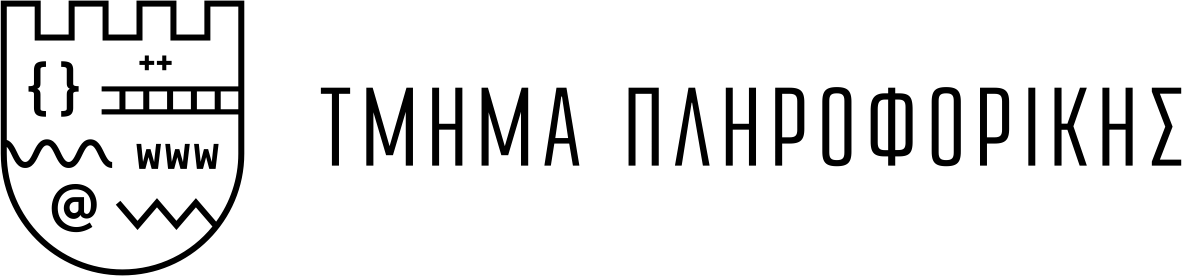
\includegraphics[width=0.5\linewidth]{logo.png}
\end{figure}
\begin{center}


\begin{figure}[h]
\centering 
%\includegraphics[width=0.3\linewidth]{authLogo.png}
\end{figure}
\begin{center}
% leave 2 cm from above text

\HRule \\[0.4cm]
{\huge Εργασία στο μάθημα της Κρυπτογραφίας}

\HRule \\[0.4cm]
\end{center}

% put this on the bottom
\vfill
\begin{doublespacing}

{\LARGE 
Καλαθάς Μάνος - ΑΕΜ:101 \par}

\vfill 
{\Large \today}
\end{doublespacing}
\end{center}
\end{titlepage}

% insert table of contents
\tableofcontents

\clearpage

% leave blank page before main part
\blankpage

\section{Άσκηση 1.3}
Ξεκινάω και ελέγχω για όλες τις τιμές του εκθέτη το αποτέλεσμα της έκφρασης \(g^{ab} \mod{677}\) και τυπώνω τις τιμές του εκθέτη που δίνουν αποτέλεσμα 1.

\section{Άσκηση 2.4}
Υπολογίζω αρχικά την τιμή του \lt{modulo} και πραγματοποιώ γρήγορη ύψωση σε δύναμη για να υπολογίσω τους τρεις παράγοντες modulo την τιμή που βρήκαμε, χρησιμοποιώντας την ιδιότητα \( a\cdot b \mod{c} = a \mod{c} \cdot b \mod{c} \) και τους πολλαπλασιάζω με τον αλγόριθμο Karatsuba.

\section{Άσκηση 3.1}
Υποθέτω ότι οι αριθμοί της μορφής \(4n+3\), \(n \in \mathbb{Z} \) είναι τέλεια τετράγωνα. Μπορούν άρα να γραφούν ως: 
$$4n+3 = x^2 $$
Το πρώτο μέρος της εξίσωσης είναι ένας περιττός αριθμός άρα και τα \(x^2,x\) είναι και αυτοί περιττοί, άρα: \(x = 2k+1\), \(k \in \mathbb{Z} \). Αντικαθιστώντας στην αρχική εξίσωση έχω ότι:
$$4n+3 = (2k+1)^2 \iff 4n+3 = 4k^2 + 4k + 1 \iff 4k^2 + 4k - 4n = 2 \iff 2(k^2 + k - n) = 1 \quad k,n \in \mathbb{Z}$$
Καταλήξαμε λοιπόν σε άτοπο άρα και η αρχική υπόθεση είναι λανθασμένη.\\

Για το δεύτερο ερώτημα, αρκεί να αποδείξω ότι όλοι οι αριθμοί 11,111,1111 μπορούν να γραφούν σαν 4n+3 και από την παραπάνω απόδειξη προκύπτει ότι οι αριθμοί που εξετάζουμε δεν μπορεί να είναι τέλεια τετράγωνα. Παρατηρώ ότι μπορώ να γράψω 111 = 100 + 11, 1111 = 1000 + 11, 11111 = 10000 + 11 κ.ο.κ. Έστω ότι επιλέγω χ έναν τυχαίο όρο από την ακολουθία, ισχύει ότι:
\begin{align}
    \congruence{x}{11}{100} \iff x = 100 \cdot k + 11 \iff x = 4 ( 25 \cdot k) + 11 \\ \notag
    \iff \congruence{x}{11}{4} \iff \congruence{x}{3}{4} \notag
\end{align}
Από τον ορισμό του modulo έχω \(χ = 4n + 3, n \in \mathbb{Z}\) Ο.Ε.Δ.

\section{Άσκηση 3.4}
Έστω ότι το \(2^m\) είναι άθροισμα διαδοχικών ακέραιων αριθμών τότε μπορώ να το γράψω σαν: $$2^m = a_i+...+a_k = ka_i + \frac{k(k+1)}{2} = \frac{2 \cdot k \cdot a_i + k^2 + k}{2} \iff 2^{m +1 } = k(2\cdot a_i + k + 1)$$
Αλλά ο όρος \(2^{m+1}\) αποτελείται μόνο από ζυγούς παράγοντες άρα πρέπει και το δεύτερο μέρος της εξίσωσης να ικανοποιεί την ίδια ιδιότητα. Εξετάζω δύο περιπτώσεις: \begin{itemize}
    \item Ο k είναι περιττός, άρα αυτομάτως καταλήγουμε σε άτοπο.
    \item Ο k είναι ζυγός, επομένως και το \(2\cdot a_i + k + 1\) είναι ένας άρτιος αριθμός συν ένα, άρα και περιττός που οδηγεί πάλι σε άτοπο.
\end{itemize}
Το \(2^m\) επομένως δεν μπορεί να είναι άθροισμα διαδοχικών ακέραιων αριθμών.

\section{Άσκηση 3.25}
Έστω ότι ο $\sqrt{p}$ είναι ρητός, τότε \(\sqrt{p} = \frac{q}{n}, \iff p = \frac{q^2}{n^2} \iff n^2p = q^2 \quad q,n \in \mathbb{N}\) \\
Από το θεμελιώδες θεώρημα αριθμητικής έχω:
$$
χ = p_1^{a_1}\cdot...\cdot p_n^{a_n}
$$
Τα τέλεια τετράγωνα, επομένως και τα $q^2,n^2$ έχουν άρτιο αριθμό πρώτων στην παραγοντοποίηση τους. Στον όρο $n^2 \cdot p$ το p είτε είναι παράγοντας του n ή όχι και αντιστοίχως εμφανίζεται συνολικά \(\#p=1\) ή \(\#p=2κ+1,  k \in \mathbb{N}\) φορές στο πρώτο μέρος της εξίσωσης που είναι ένας περιττός αριθμός άρα καταλήγουμε σε άτοπο. Επομένως ο p δεν μπορεί να είναι ρητός.

\section{Άσκηση 3.28}
Χρησιμοποιώ τον εκτεταμένο αλγόριθμο του Ευκλείδη, βρίσκω αρχικά τον gcd(540,315):
\begin{align*}
&540 = 315 + 225 \notag \\
&315 = 225 + 90 \notag \\
&225 = 2\cdot90 + 45 \notag \\
&90 = 2\cdot45 \notag 
\end{align*}
Και μετά τους παράγοντες Bezout:
\begin{align*}
45 = 225 - 2\cdot90 = 225 - 2(315 - 225) = \notag \\
= -2\cdot315 + 3\cdot225 = -2\cdot315 + 3(540 - 315) = 3\cdot540 -5\cdot315 \notag
\end{align*}
Άρα α=3 και β=-5 και ισχύει $$3\cdot540 -5\cdot315 = 45$$

\section {Άσκηση 3.30}
Ισχύει gcd(a,b)=1 άρα \(ax + by = 1\) και οι a,b είναι πρώτοι μεταξύ τους:
\begin{enumerate} 
\item Με την λογική, ο μέγιστος κοινός διαιρέτης του c και του b θα είναι ο ίδιος με αυτόν του ac και b αφού οι a και b είναι πρώτοι μεταξύ τους και άρα το a δεν προσθέτει κάποιο διαιρέτη για να αλλάξει το αποτέλεσμα.
Διατυπώνοντας το μαθηματικά, έστω ότι έχουμε:
\begin{align*}
    gcd(ac,b) = p \Rightarrow p | ac \land p | b \Rightarrow p | c \land p | b \Rightarrow p | gcd(c,b) \Rightarrow p | q\\
    gcd(c,b) = q \Rightarrow q | c \land q | b \Rightarrow q | ac \land  q | b \Rightarrow q | gcd(ac,b) \Rightarrow q | p
\end{align*}
Για το βήμα \(p|ac \Rightarrow p|c\), χρειάζεται να ξέρουμε ότι gcd(p,a)=1 κάτι που ισχύει διότι ο p θα είναι είτε ένα είτε κάποιος διαιρέτης του b αλλά οι a και b είναι πρώτοι μεταξύ τους άρα και κανένας διαιρέτης του p δεν θα διαιρεί τον α. 
Από τις δύο προηγούμενες προτάσεις επομένως, ισχύει ότι \(p=q \Rightarrow gcd(ac,b)=gcd(c,b)\) Ο.Ε.Δ.

\item Έστω gcd(a+b, a-b) = g, τότε:
\begin{align*}
    g | a+b \Rightarrow gx = a+b \\
    g | a-b \Rightarrow gy = a-b
\end{align*}
Προσθέτοντας και αφαιρώντας κατά μέλη έχουμε:
\begin{align*}
    g(x+y) = 2a \Rightarrow g | 2a\\
    g(x-y) = 2b \Rightarrow g | 2b
\end{align*}
Όμως οι a,b είναι πρώτοι μεταξύ τους οπότε δεν έχουν κοινό διαιρέτη, άρα πρέπει το g να είναι είτε ένα ή δύο διότι αλλιώς το g θα διαιρούσε και τα a,b κάτι αδύνατο.
Αν a,b περιττοί τότε οι a+b,a-b είναι ζυγοί αριθμοί και χρησιμοποιώντας το προηγούμενο εύρημα καταλήγουμε στο ότι ο μέγιστος κοινός διαιρέτης τους είναι το 2.

\item Αρκεί να αποδείξω ότι \(p = gcd(2^a-1, 2^b-1)\) είναι πρώτοι μεταξύ τους.Οι αριθμοί \(2^a-1, 2^b-1\) είναι περιττοί άρα όλοι οι παράγοντες τους και επομένως και το p είναι περιττοί αριθμοί. Έχω ότι:
\begin{align*}
    p | 2^a-1, \quad p | 2^b-1 \Rightarrow p | 2^a - 2^b - 2, \quad p | 2^a + 2^b
\end{align*}

\item Από το προηγούμενο ερώτημα συμπεράναμε ότι άν \\ \(gcd(a, b) = 1 \Rightarrow gcd(2^a - 1,2^b -1) =1\). Για το ζητούμενο αρκεί να αποδείξουμε ότι gcd(p, q) = 1 κάτι που ισχύει αφού όλοι οι πρώτοι αριθμοί είναι και πρώτοι με όλους τους άλλους ακέραιους άρα και \(gcd(M_p, M_q)=1\).
\end{enumerate}

\section {Άσκηση 3.39}
Για να βρούμε το άθροισμα τον θετικών διαιρετών ενός αριθμού ξεκινάμε από το 2 μέχρι την τιμή της ρίζας του και ελέγχουμε αν το υπόλοιπο της διαίρεσης είναι μηδέν. Σε αυτήν την περίπτωση κρατάμε τον διαιρέτη και το πηλίκο και τα προσθέτουμε στο άθροισμα των διαιρετών. Έπειτα, ελέγχουμε για κάθε ακέραιο στο διάστημα \([2, 10^{7}]\) αν ισχύει η ανισότητα
\(\sigma(n) > e^{\gamma}n\ln{(\ln{n})}\), με τον μεγαλύτερο αριθμό για τον οποίο αληθεύει να είναι ο 5040.

\section {Άσκηση 3.74}
Έχουμε το σύστημα:
\begin{align}
    \begin{cases}
    &\congruence{2x}{1}{5} \notag \\ 
    &\congruence{3x}{9}{6} \notag \\
    &\congruence{4x}{1}{7} \notag \\
    &\congruence{5x}{9}{11} \notag 
    \end{cases}
\end{align}
Έστω ότι \(n_1=1,n_2=9,n_3=1,n_4=9\) και \(m_1=5,m_2=6,m_3=7,m_4=11\) άρα \(M = m_1 \cdot m_2 \cdot m_3 \cdot m_4 = 2310\) και \(M_1 = \frac{M}{m_1} = 462, M_2 = \frac{M}{m_2} = 385, M_3 = \frac{M}{m_3} = 330, M_4 = \frac{M}{m_4} = 210\),  με όλα τα ζεύγη των m να είναι πρώτοι μεταξύ τους άρα μπορώ να εφαρμόσω το κινέζικο θεώρημα υπολοίπων.
Επομένως έχω ότι:
\begin{align}
   x = \sum_{i=1}^{4} M_i υ_i n_i = 
   462 \cdot υ_1 \cdot 1 + 385 \cdot υ_2 \cdot 9+ 330 \cdot υ_3 \cdot 1 + 210 \cdot υ_4 \cdot 9
\end{align}
Βρίσκω τα \(υ_i =\congr{{M_i}^{-1}}{m_i}\) από τον ευκλείδειο αλγόριθμο με τιμές \(υ_1 = 3, υ_2 = 1, υ_3 = 1, υ_4 = 1\). Αντικαθιστώντας στην (6.1) έχουμε:
\begin{align}
    x = 462 \cdot 3 \cdot 1 + 385 \cdot 1 \cdot 9 + 330 \cdot 1 \cdot 1 + 210 \cdot 1 \cdot 9 = 7071 \pmod*{2310} = 141 
\end{align}

\section {Άσκηση 4.41}
Βρίσκω αρχικά τον αριθμό Fibonacci \(F_{104911}\) και αφού υλοποιήσω τον αλγόριθμο Miller-Rabin φτιάχνω μία συνάρτηση που να υπολογίζει γρήγορα μεγάλες δυνάμεις με modulo χρησιμοποιώντας την δεξιά προς τα αριστερά δυαδική μέθοδο και αποδεικνύεται ότι ο αριθμός που ελέγχω είναι πράγματι πρώτος.

\section {Άσκηση 4.46}
Παράγω αρχικά με τη βοήθεια της βιβλιοθήκης random τυχαίους αριθμούς και θέτω το πρώτο και το τελευταίο δυαδικό στοιχείο τους ίσο με την μονάδα ώστε να είναι περιττοί και μήκους 2048 bit.
Έστω p ένας τυχαίος αριθμός, θα ελέγξω στην περίπτωση που είναι πρώτος, αν και κάποιος από τους \( q = 2*p + 1, z = (p - 1)/2\) είναι και αυτοί πρώτοι άρα και θα έχω ένα ζεύγος Sophie-Germain πρώτων.
Ελέγχω πρώτα με ένα fermat test αν οι αριθμοί είναι πρώτοι λόγω υψηλότερης ταχύτητα και μετά επαληθεύω με το τεστ Miller-Rabin αξιωποιώντας και την ιδιότητα του lazy evaluation της python για καλύτερη απόδοση.

\section {Άσκηση 6.3}
Εφόσον το Ν είναι μικρό μπορούμε να το παραγοντοποιήσουμε βρίσκοντας έτσι τους πρώτους p,q άρα και το φ(Ν). Έπειτα, από την ισοδυναμία \congruence{e\cdot d}{1}{\phi(Ν)} και έχοντας το e βρίσκουμε το ιδιωτικό κλειδί d και εύκολα αποκρυπτογραφούμε το μήνυμα καταλήγοντας στην έκφραση "welcowe to the real world".

\section {Άσκηση 6.5}
Έστω \(p = 5, q = 11, N = 55, c = 14\), τότε: 
\begin{align}
    &F^{-1}(sk, y) : \congruence{x^2} {15}{55} \notag
\end{align}
Λύνω το σύστημα:
\begin{align}
    \begin{cases}
        & \congruence{x^2}{4}{5} = 4 \notag \\
        & \congruence{x^2}{14}{11} = 3 \notag \\
    \end{cases}
\end{align}
Η τετραγωνική ρίζα του 4\(\pmod*{5}\) είναι το 2, ενώ του \(3\pmod*{11}\) το 5, άρα λύνω το σύστημα:
\begin{align}
    \begin{cases}
        & \congruence{x}{2}{5} \notag \\
        & \congruence{x}{5}{11}\notag \\
    \end{cases}
\end{align}
Εφαρμόζω το Κινέζικο Θεώρημα αφού οι 5 και 11 είναι πρώτοι μεταξύ τους και έχω: 
\begin{align*}
   & m = 55, m_1 = 5, m_2 = 11, M_1 = \frac{m}{m_1} = 11, M_2 = \frac{m}{m_2} = 5, \notag \\
   & \congruence{υ_1}{M^{-1}_1}{m_1} = 1\pmod*{5}, \\ \notag
   & \congruence{υ_2}{M^{-1}_2}{m_2} = 9\pmod*{11} \notag
\end{align*}
Άρα έχουμε τις τέσσερις πιθανές λύσεις που δίνονται από τον τύπο:
\begin{align}
    \congruence{x}{(\pm{2}\cdot M_1 \cdot υ_1 \pm{5}\cdot M_2 \cdot υ_2)}{55} = 23, \textbf{12}, 22, 43 \notag
\end{align}
Αλλά ξέρουμε ότι ισχύει m < 20 άρα m = 12.

\section {Άσκηση 7.2}
Βρίσκω αρχικά το ιδιωτικό κλειδί με τιμή 20882 από την επίθεση Wiener. Στη συνέχεια, αποκρυπτογραφώ το μήνυμα που είναι σε μορφή base64 που μου δίνει ένα string. Αφού υποστεί επεξεργασία δίνεται μία σειρά από κρυπτογραφημένα με RSA νούμερα τα οποία εύκολα μπορούμε να αποκρυπτογραφήσουμε αφού έχουμε το ιδιωτικό κλειδί από πριν, καταλήγοντας στο μήνυμα `` Just because you are a character doesn't mean that you have character''.

\section{Άσκηση 10.1}
Για την παραγωγή ενός ζεύγους δημόσιου/ιδιωτικού κλειδιού χρησιμοποιούμε την παρακάτω εντολή και ακολουθούμε τις οδηγίες που μας δίνονται:
\begin{lstlisting}
gpg --gen-key
\end{lstlisting}

Για να δούμε όσα κλειδιά έχουμε στην διάθεση μας:
\begin{lstlisting}
gpg --list-keys
\end{lstlisting}

Για να εξάγουμε ένα δημόσιο κλειδί ώστε να το διανέμουμε εκτελούμε την εντολή:
\begin{lstlisting}
gpg --export recipient@gmail.com > pubkey.asc
\end{lstlisting}

Για να εισάγουμε το δημόσιο κλειδί που έχουμε λάβει από κάποιον άλλο κάνουμε:
\begin{lstlisting}
gpg --import pubkey.asc
\end{lstlisting}

Για την κρυπτογράφηση ενός μηνύματος:
\begin{lstlisting}
gpg --encrypt --recipient recipient@gmail.com message.txt
\end{lstlisting}

Για την αποκρυπτογράφηση ενός μηνύματος:
\begin{lstlisting}
gpg --decrypt message.txt.gpg
\end{lstlisting}

\bibliographystyle{plain}
\bibliography{bib.bib}

\end{document}